
%(BEGIN_QUESTION)
% Copyright 2006, Tony R. Kuphaldt, released under the Creative Commons Attribution License (v 1.0)
% This means you may do almost anything with this work of mine, so long as you give me proper credit

What is a valve {\it actuator}?  What does it mean if a sliding-stem valve actuator is {\it reverse-acting}?  How does this compare with a {\it direct-acting} actuator?

\underbar{file i00779}
%(END_QUESTION)





%(BEGIN_ANSWER)

A valve {\it actuator} is the mechanism that moves the valve stem or shaft in response to a control signal, usually compressed air.

\vskip 10pt

A {\it reverse-acting} valve actuator is one where the actuating stem retracts into the actuator (pulls up from the valve body) when air pressure is applied:

$$\includegraphics[width=15.5cm]{i00779x01.eps}$$

By contrast, a {\it direct-acting} actuator extends its stem (pushes into the valve body) when air pressure is applied:

$$\includegraphics[width=15.5cm]{i00779x02.eps}$$

%(END_ANSWER)





%(BEGIN_NOTES)

Actuators come in a variety of forms, usually pneumatic in nature.  However, hydraulic and electric actuators exist as well, with certain advantages and disadvantages in comparison to the more common pneumatic designs.

One way I use to remember the direct/reverse relationship is by simplicity of design.  The direct-acting actuator requires no seal around the stem, and is therefore simpler than the reverse-acting actuator.  When you see the word, ``direct,'' think {\it simple}.

%INDEX% Final Control Elements, valve: direct-acting and reverse-acting actuator

%(END_NOTES)


